\documentclass[twoside,11pt,openright]{report}

\usepackage[latin1]{inputenc}
\usepackage[american]{babel}
\usepackage{a4}
\usepackage{latexsym}
\usepackage{amssymb}
\usepackage{amsmath}
\usepackage{epsfig}
\usepackage[T1]{fontenc}
\usepackage{lmodern}
\usepackage[labeled]{multibib}
\usepackage{color}
\usepackage{datetime}
\usepackage{epstopdf} 

\renewcommand*\ttdefault{txtt}

\newcommand{\todo}[1]{{\color[rgb]{.5,0,0}\textbf{$\blacktriangleright$#1$\blacktriangleleft$}}}

\newcites{A,B}{Primary Bibliography,Secondary Bibliography}

% see http://imf.au.dk/system/latex/bog/

\begin{document}

%%%%%%%%%%%%%%%%%%%%%%%%%%%%%%%%%%%%%%%%%%%%%%%%%%%%%%%%%%%%%%%%%%%%%%%

\pagestyle{empty} 
\pagenumbering{roman} 
\vspace*{\fill}\noindent{\rule{\linewidth}{1mm}\\[4ex]
{\Huge\sf Computation of Edit Distance in Compressed Strings}\\[2ex]
{\huge\sf Kasper Nielsen, 20091182}\\[2ex]
\noindent\rule{\linewidth}{1mm}\\[4ex]
\noindent{\Large\sf Master's Thesis, Computer Science\\[1ex] 
\monthname\ \the\year  \\[1ex] Advisor: Christian N�rgaard Storm Pedersen\\[15ex]}\\[\fill]}

\epsfig{file=logo.eps}\clearpage

%%%%%%%%%%%%%%%%%%%%%%%%%%%%%%%%%%%%%%%%%%%%%%%%%%%%%%%%%%%%%%%%%%%%%%%

\pagestyle{plain}
% \chapter*{Abstract}
% \addcontentsline{toc}{chapter}{Abstract}

% \todo{in English\dots}

% \chapter*{Resum\'e}
% \addcontentsline{toc}{chapter}{Resum\'e}

% \todo{in Danish\dots}

% \chapter*{Acknowledgements}
% \addcontentsline{toc}{chapter}{Acknowledgments}

% \todo{\dots}

% \vspace{2ex}
% \begin{flushright}
%   \emph{Kasper Nielsen,}\\
%   \emph{Aarhus, \today.}
% \end{flushright}

\tableofcontents
\pagenumbering{arabic}
\setcounter{secnumdepth}{2}

%%%%%%%%%%%%%%%%%%%%%%%%%%%%%%%%%%%%%%%%%%%%%%%%%%%%%%%%%%%%%%%%%%%%%%%

%\chapter{Introduction}
%\label{ch:intro}
%\todo{\dots}

\section{Introduction}
Focus on computation of edit distance. That is, insert / delete of cost 1, match of cost 0. This can be generalized to different classes of scoring functions, which in some cases results in more complicated algorithms with worse asymptotic running time and space consumption, even if the cost function is assumed to be computable in constant time.

Focus on how well strings can be compressed as SLPs, compared to other encodings ex BWT and entropy based compression algorithms (ex Huffman encoding). Try to think about algorithms that works for these other (presumably better) compression algorithms.

\section{Compression of strings}
Describe and discuss different types of string compression.
\begin{itemize}
  \item Information theoretical bound for compression, and encoding schemes satisfying this bound (ex Huffman encoding / Arithmetic coding).
  \item Definition of SLPs, and compression schemes transformable to SLPs (Z77, Z78, LZW).
  \item Other transformations possibly making subsequent compression more efficient (ex BWT)
  \item Compare how well the strings are compressed compared to the information theoretic lower bound given by the entropy.
\end{itemize}

\section{Simpel}
\todo{Give credit to some guy!}
A standard dynamic programming algorithm for solving the Edit Distance problem, is denoted the simple algorithm or simple implementation. It is given two string $A[1..n]$ and $B[1..m]$ for which the edit distance should be computed, and fills out a matrix of size $n \times m$ where a given entry $(i, j)$ corresponds to the edit distance between $A[1..i]$ and $B[1..j]$. The rules for filling out a table entry follows directly from the definition of edit distance when extending a string, and are as follows:
\todo{match, insert, delete}
The base case where a string is aligned to the empty string is trivially $0$. Therefore the edit distance between two string can be computed using both $O(nm)$ time and space. Notice that an easy optimization where only the last row used is stored in memory reduces the space consumption to $O(\min\{n, m\})$.

\subsection{Backtracking}
If the actual alignment(s) of the strings is desirable, it can be found by a standard back-tracking approach on the computed matrix.

This however implies that the simple space optimization from before does not work, as all entries in the computed table potentially is needed for the backtracking. However, a divide-and-conquer algorithm was given by Hirshberg\todo{Cite} that reduces the space consumption of $O(\min\{n, m\})$ without asymptotically increasing the running time.\todo{Describe the approach?}

\subsection{Optimizations}
Ideas:
\begin{itemize}
  \item Compute matrix only around its diagonal, and then extend if needed.
  \item Using SIMD instructions.
  \item Parallelization (CPU / GPU).
\end{itemize}

\section{Compression based algorithms}
A recent approach for speeding up the computation of edit distance, is to do some compression of the strings before aligning them, and then in some way do the edit distance computation using the compressed strings, which in many cases will be shorter than the original input.

\subsection{The 4 Russian Trick}
This approach was not originally presented as a compression based algorithm, but using that each entry in the dynamic programming matrix is changing at most 1 from an adjacent entry, and that the alphabet is finite, it is possible to encode blocks of the matrix space efficiently and pre-compute all of them. That is, for all different sub-strings and possible inputs to compute the relative outputs when applying the block. This is then used to fill out the original dynamic programming matrix block-by-block.
\todo{Describe details and analyze time complexity?.}

\subsection{Run-Length Encoding}
\begin{itemize}
  \item \todo{Describe RLE}
  \item Not the focus / implemented in this thesis, but the result is included for completeness. Refer old thesis for experimental results of this approach?
  \item \todo{cite} gave an algorithm running in time $O(nm)$ where $n$ and $m$ denotes the size of the compressed sequences. This is the first result where the running time is only depending on the length of the compressed strings. However, for string not containing long runs of the same symbol, RLE will generate strings longer than the original input!
\end{itemize}

\subsection{Compression based on SLPs}
This is the main focus of this thesis.

\newcommand{\SLP}[1] {\mathcal{#1}}

The algorithm is a bit like the 4 Russion Algorithm, however the blocking of the dynamic programming table is based on the productions of the SLPs, so that reused productions results in reusable blocks. The algorithm can be summarized in the following steps:
\begin{itemize}
  \item Construct a SLP representation $\SLP{A}$, $\SLP{B}$ of the two input strings $A$ and $B$. The better the compression scheme is able to compress the SLP representations the faster the algorithm will be. The running time of this scheme depends on the compression scheme employed, but using Z77, Z78 or LZW this can be in time $O(N)$ \todo{be sure, and cite?}.
  \item Select productions from the SLPs generating strings of length $O(x)$ for some fixed $x$ are selected in such a way that they cover the entire string without duplication. This can trivially be done in time $O(N)$ where also a list of selected productions is generated in such a way that the associated strings is the original input string.
  \item Blocks from the dynamic programming table (called DIST tables) are precomputed for all the selected productions. These DIST tables naively takes up can be represented using $O(x^2)$ space to represent, but using a succinct representation given in \todo{cite}, it is possibly to reduce the space consumption to $O(x)$ trading for a query-time of $\log^2 x$ time. This increased query time is also the reason the algorithm gains an extra $\log{x}$ factor, which is conjectured to be unnecessary \todo{cite}. Using the succinct representation and a the way of merging succinct DISTs from \todo{cite}, this step can be computed in time $O(n^2x\log{x})$.
  \item The dynamical programming table is filled up by using the generated partition of the string and then applying the DIST tables. This step takes time $O(\left(\frac{N}{x}\right)^2 \cdot AP(x))$ where $AP(x)$ is the time to apply a DIST table. Using the succinct representation, \todo{cite} shows how to make $AP(x) = x\log{x}$, leading to a total running time of $O(\frac{N}{x} \log{x})$.
\end{itemize}

\subsubsection{Selection of productions}
Each of the SLPs are blocked individually using the same algorithm.
\begin{itemize}
  \item First the SLP is traversed bottom up, where all productions are annotated with the derived string length, and if the derived string is of length less than $2x$, the string is associated to the production. A production is marked as a \textit{key production} iff it derives a string of length greater than $x$ and both of its children derived strings of length strictly less than $x$. All these key productions are selected, which covers some part of the string.
  \item In order to cover the rest of the input strings, the path between two key productions is traversed, and all nodes in between are merged to obtain strings of length $O(x)$ (notice that this is possible since there can be no key productions in between, that is, all derived strings associated to some production has a length smaller than $x$) \todo{Figure, or refer to paper?}. The procedure works by traversing the path and then concatenating strings until one with sufficient length is generated. This string is then associated to the last production seen on the path.
  \item Notices that the beginning and end of the string is special cases. But they can be handled by exactly the same procedure.
  \item Due to the bottom up nature, a repeated production in two parts of the string will result in the same selected productions. This is very important in obtaining the desired speedup!
  \item Notice that a given production is only associated one unique string. For the key productions this is trivial, and for the second type it follows since the same key productions are selected in different parts of the strings, resulting in the paths between the key productions being unique, so that they always produces the same result.
\end{itemize}

\subsubsection{Building DIST repository}
Build by recursively merging DIST tables for sub-productions of the selected productions. Notice that generating DIST tables for a pair of terminals is trivial.
\begin{description}
  \item[Productions associated with entires string the derive] This is the case for all key productions. Say a DIST table needs to be constructed for two non-terminals $a$ and $b$. Call the left and right child of the productions respectively $a_L$, $a_R$, $b_L$ and $b_R$. The DIST table is constructed by first recursively constructing the DIST tables for all combinations of the children, ie. $(a_L, b_L), (a_L, b_R), (a_R, b_L)$ and $(a_R, b_R)$. Then the DIST from $a$ and $b$ can be obtained by merging as shown in Figure~\ref{fig:compression:dist:merge}.
  \begin{figure}
    \centering
    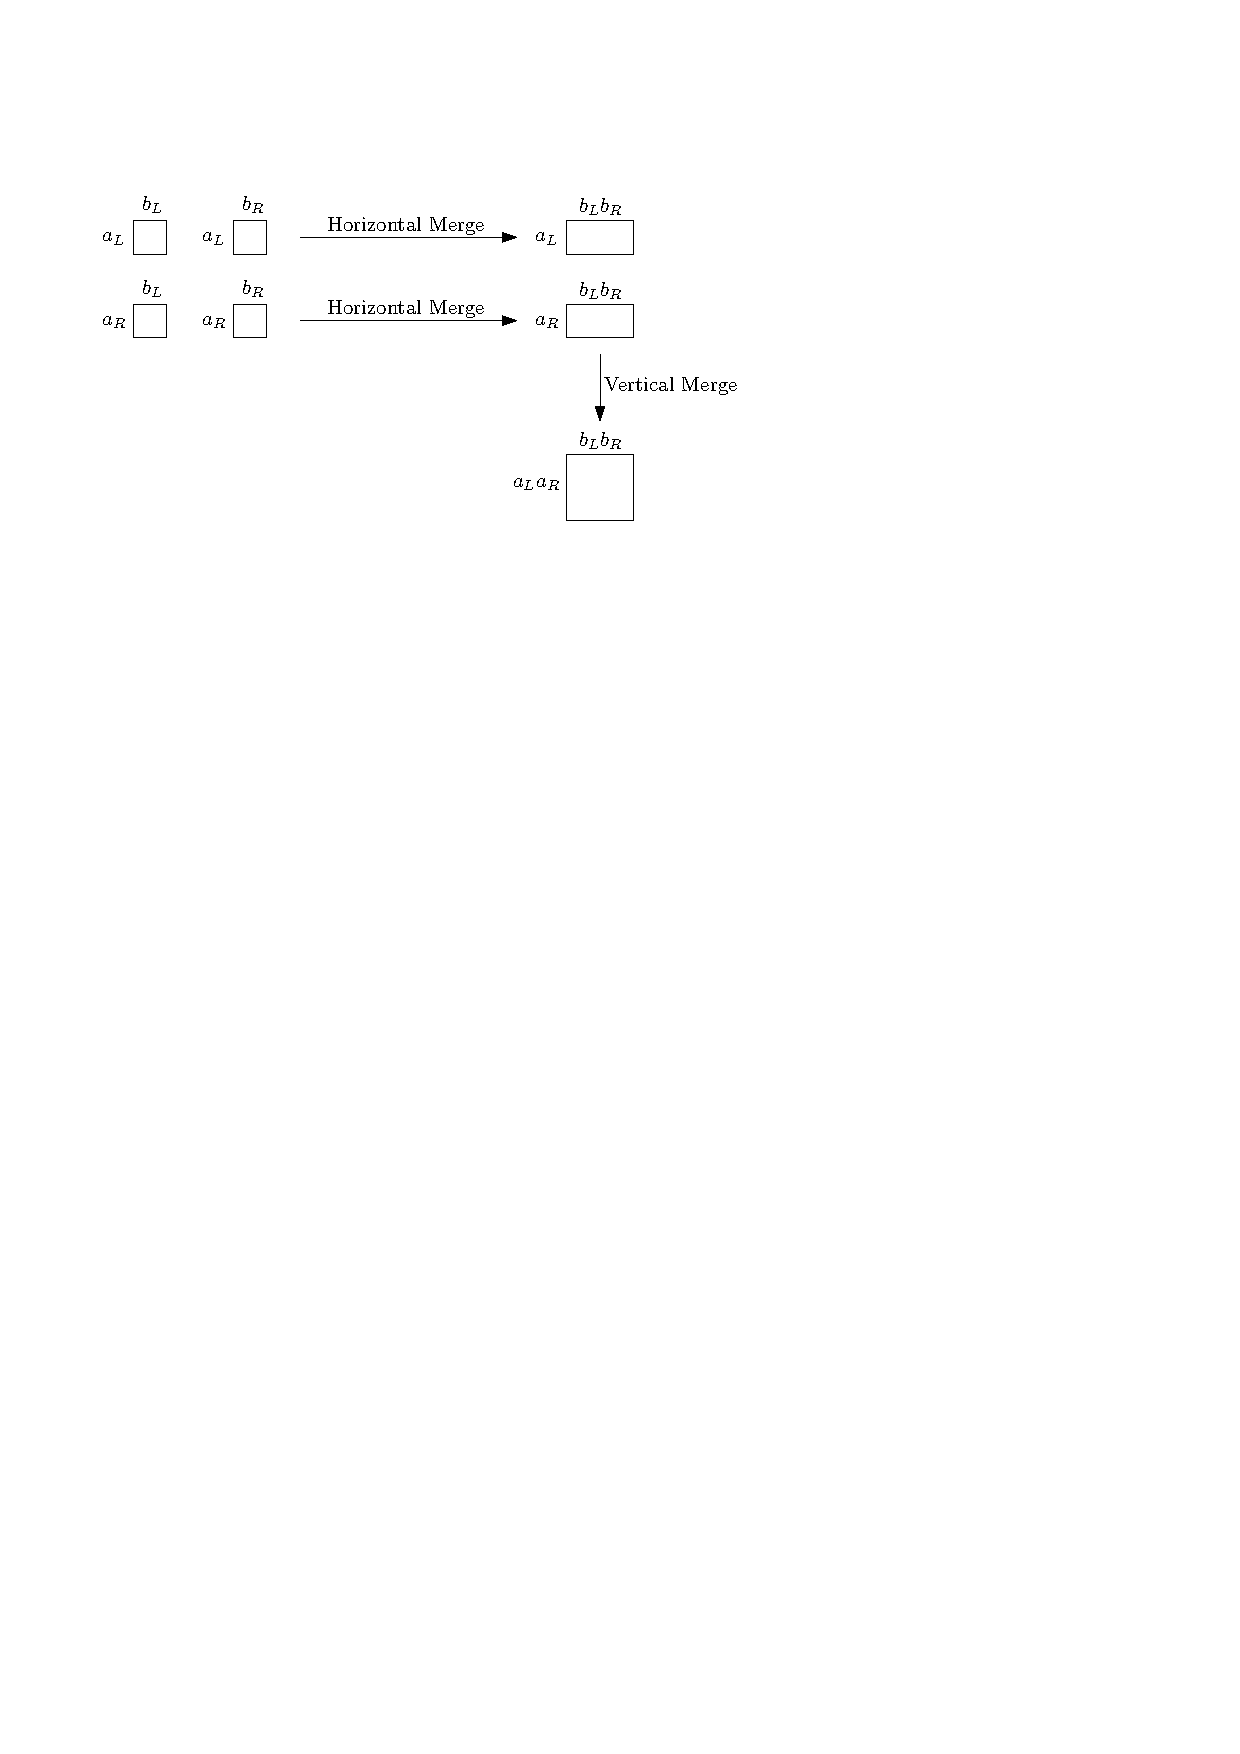
\includegraphics{images/dist_merge}
    \caption{Merging phases of DIST tables from the children to obtain the DIST for the concatenated strings.}
    \label{fig:compression:dist:merge}
  \end{figure}

  \item[Productions associated with substring] For this type of productions a merging approach is also employed. Depending on what side of the path the node was selected, its left/right child is chosen accordantly, and then they are recursively solved and merged together as in the previous case.
\end{description}
Since the number of productions is bounded by $O(n^2)$, the time for constructing the dist repository can be build in time $O(n^2 M(x))$ using memorization, where $M(x)$ denotes the time for merging two DIST tables, which for a rational scoring function and the succinct DIST representation takes time $O(x \log{x})$. In total $O(n^2x\log{x})$ time is spend.

\subsubsection{Filling out the dynamical programming table}
The dynamical programming table is filled from top to bottom, left to right. This is done by keeping two columns of the table in memory (could be reduced to a little more than one column), and then $O(x)$ of a row. This specifies the inputs $I$ to the dist table, and the output can then be computed by
\[
  O[j] = \min_i \{ I[i] + DIST[i, j] \},
\]
since the DIST table stores the shortest path from input $i$ to output $j$. Evaluating the above formula directly for every input takes $O(x^2)$ time, which is too much. However using the succinct representation of the DIST tables, \todo{cite} described how it can be evaluated in time $O(x\log{x})$.

Alternatively if a simple representation of the DIST tables is used, then it can be evaluated in time $O(x)$ using the SMAWK algorithm (however, this would increase the time needed for constructing the dist tables).

%%%%%%%%%%%%%%%%%%%%%%%%%%%%%%%%%%%%%%%%%%%%%%%%%%%%%%%%%%%%%%%%%%%%%%%

\addcontentsline{toc}{chapter}{Bibliography}
\bibliographystyleA{plain} 
\bibliographyA{refs}
%\addcontentsline{toc}{chapter}{Secondary Bibliography}
%\bibliographystyleB{plain} 
%\bibliographyB{refs} % remove this if you don't need secondary literature

\end{document}

